\documentclass{article}

\usepackage[utf8]{inputenc}
\usepackage{mdwlist}
\usepackage[inner=3cm,outer=4cm]{geometry}
\usepackage{mathtools}

\usepackage{Sweave}
\begin{document}
\Sconcordance{concordance:HW08ZIPlogistic.tex:HW08ZIPlogistic.Rnw:%
1 7 1 1 0 23 1 1 9 8 0 5 1 3 0 1 2 2 1 1 8 10 0 1 2 2 1 1 3 2 0 3 1 4 0 %
1 3 4 1 1 2 1 0 3 1 4 0 1 2 2 1 1 3 2 0 2 1 31 0 1 1 23 0 1 1 5 0 4 1 %
14 0 1 2 11 1 1 3 2 0 2 1 31 0 1 1 23 0 1 1 5 0 2 1 4 0 1 2 3 1 1 2 1 0 %
1 2 1 0 1 1 34 0 1 2 2 1 1 3 2 0 1 1 32 0 1 2 2 1 1 3 2 0 1 1 29 0 1 2 %
2 1 1 2 10 0 1 2 5 0 1 2 4 1 1 3 7 0 1 1 5 0 1 1 5 0 2 1 1 6 8 0 1 2 3 %
1 1 2 5 0 1 2 11 1 1 3 2 0 2 1 3 0 1 2 2 1 1 3 2 0 1 1 3 0 1 2 3 1 1 3 %
2 0 2 1 31 0 1 1 23 0 1 1 5 0 2 1 3 0 1 2 8 1 1 3 2 0 1 1 13 0 1 2 3 1 %
1 4 3 0 2 1 31 0 1 1 23 0 1 1 5 0 2 1 3 0 1 2 5 1 1 3 2 0 1 3 2 0 1 1 %
34 0 1 2 3 1 1 3 2 0 1 1 32 0 1 2 3 1 1 4 3 0 1 1 29 0 1 2 3 1 1 3 11 0 %
1 2 1 0 1 1 3 0 1 2 3 1 1 3 7 0 1 1 5 0 1 1 5 0 1 2 1 0 1 1 1 5 7 0 1 2 %
4 1}


\title{Homework 08. Zero-inflated Poisson and Logistic Regression. PLS206 Fall 2014}
\author{Emilio A. Laca}
\maketitle


\section {Zero Inflated Poisson (complete)}
\subsection{Data}

This exercise uses simulated data similar to those data used in HW07F14, but vegetation type is dropped. Thus, we know the true model and whether the assumptions are met. The data simulate the number of individuals of a relatively rare mammal observed in a series of locations in East Africa. Locations were selected haphazardly. Variables measured at each location were:

\begin{description*}
  \item[nrrm] number of individuals of the relatively rare mammal seen.
  \item[river] distance to the nearest river in km.
  \item[road] distance to nearest road in km.
  \item[cover] visual cover; proportion of a vertical surface visible from 20 m.
\end{description*}

The data simulation code is presented for completeness, but for the analysis we use a preset simulation that remains constant across compilations of this document. Note that this simulation includes zero inflation.

Reading the simulation code may also help to understand the type of data specifically addressed by ZIP's. The simulation shows plainly the two processes that generate ZIP data.
First, we generate a series of values for the predictors. Arbitrarily, this values are generated independently with various suitable distributions. The parameter values used are selected so predictor values are plausible. Then, plausible parameter values for the count are set.
\begin{Schunk}
\begin{Sinput}
> dsim <- data.frame(river = round(runif(150, min=0.5, max=15),1),
+                  road = round(rchisq(150, 6),1),
+                  cover = c(
+                    rbeta(30,2,10),
+                    rbeta(30,4,8),
+                    rbeta(30,10,3),
+                    rbeta(30,8,4),
+                    rbeta(30,6,6)))
> beta0 <- 0.2
> bRiver <- -0.1
> bRoad <- 0.05
> bRiverRoad <- 0.02
> bCover <- 2
\end{Sinput}
\end{Schunk}

Second, we randomly generate count data representing the number of individuals in each location, assuming that the location was found or "colonized." For this, the mean of the Poisson process is a deterministic function of the predictors.

\begin{Schunk}
\begin{Sinput}
> # count component
> dsim$nrrm <- rpois(150,
+                  exp(beta0 +
+                      bRiver*dsim$river +
+                      bRoad*dsim$road +
+                      bRiverRoad*dsim$river*dsim$road +
+                      bCover*dsim$cover))
\end{Sinput}
\end{Schunk}

Third, and independently of the counts, some observations are set to zero using a binomial process. This simulates the process by which some locations are not yet found or colonized. Thus, they have zero individuals, regardless of how good they are. As a side note, consider that every observation is assumed to be independent. In reality, unless we sample locations that are sufficiently far from each other relative to the dispersal distance of the mammal, it is likely that the probabilities of colonization are spatially correlated, and that would have to be incorporated into the simulation and then into the model.

\begin{Schunk}
\begin{Sinput}
> # zero component
> gamma0 <- 10
> gamma1 <- -2
> dsim$is.zero <- rbinom(150,1,1-exp(gamma0+gamma1*dsim$road)/(1+exp(gamma0+gamma1*dsim$road)))
> dsim$nrrm <- dsim$nrrm*dsim$is.zero
> # write.csv(dsim,"../Examples/zeroinfl.txt")
\end{Sinput}
\end{Schunk}

\subsection{Data exploration}

A plot of the table of values suggests zero-inflation.

\begin{Schunk}
\begin{Sinput}
> d1 <- read.csv("../Examples/zeroinfl.txt", header=TRUE)
> library(car)
> library(ggplot2)
> plot(table(d1$nrrm))
\end{Sinput}
\end{Schunk}
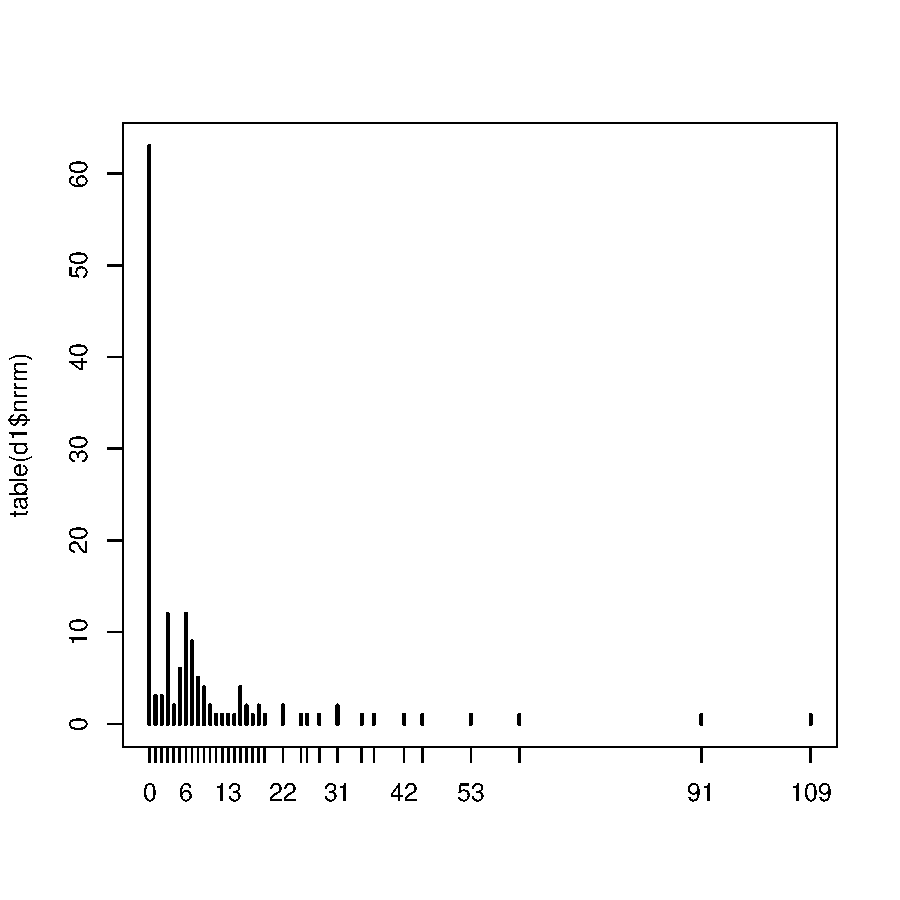
\includegraphics{HW08ZIPlogistic-004}

The number of individuals counted is a positive discrete variable. There is no limit to the potential number of individuals found. We start with a distribution that accommodates both properties, the Poisson distribution. We must take into account the fact that there are 100 observations, thus, we should not consider models with more than 15 degrees of freedom, which should not be a problem in this case.

\begin{Schunk}
\begin{Sinput}
> glm1 <- glm(nrrm ~ river + road + cover + river:road + river:cover +
+               road:cover, family=poisson, data=d1)
> plot(log(d1$nrrm+1)~log(fitted(glm1, type="response")+1))
> summary(glm1)
\end{Sinput}
\begin{Soutput}
Call:
glm(formula = nrrm ~ river + road + cover + river:road + river:cover + 
    road:cover, family = poisson, data = d1)

Deviance Residuals: 
    Min       1Q   Median       3Q      Max  
-3.4400  -1.7052  -0.6972   0.8537   3.6625  

Coefficients:
            Estimate Std. Error z value Pr(>|z|)    
(Intercept) -0.68728    0.31990  -2.148  0.03168 *  
river       -0.03273    0.03044  -1.075  0.28225    
road         0.10379    0.02047   5.072 3.94e-07 ***
cover        1.25168    0.46870   2.671  0.00757 ** 
river:road   0.01531    0.00220   6.961 3.37e-12 ***
river:cover  0.01423    0.03622   0.393  0.69432    
road:cover   0.05432    0.03229   1.682  0.09256 .  
---
Signif. codes:  0 ‘***’ 0.001 ‘**’ 0.01 ‘*’ 0.05 ‘.’ 0.1 ‘ ’ 1

(Dispersion parameter for poisson family taken to be 1)

    Null deviance: 2546.64  on 149  degrees of freedom
Residual deviance:  395.63  on 143  degrees of freedom
AIC: 755.57

Number of Fisher Scoring iterations: 5
\end{Soutput}
\begin{Sinput}
> anova(glm1, test="Chisq")
\end{Sinput}
\begin{Soutput}
Analysis of Deviance Table

Model: poisson, link: log

Response: nrrm

Terms added sequentially (first to last)


            Df Deviance Resid. Df Resid. Dev  Pr(>Chi)    
NULL                          149    2546.64              
river        1   351.94       148    2194.70 < 2.2e-16 ***
road         1  1390.02       147     804.68 < 2.2e-16 ***
cover        1   347.14       146     457.53 < 2.2e-16 ***
river:road   1    58.77       145     398.76 1.768e-14 ***
river:cover  1     0.28       144     398.48   0.59527    
road:cover   1     2.85       143     395.63   0.09164 .  
---
Signif. codes:  0 ‘***’ 0.001 ‘**’ 0.01 ‘*’ 0.05 ‘.’ 0.1 ‘ ’ 1
\end{Soutput}
\begin{Sinput}
> 1-pchisq(deviance(glm1),143) # excessive deviance; model needs to be improved
\end{Sinput}
\begin{Soutput}
[1] 0
\end{Soutput}
\begin{Sinput}
> par(mfrow=c(2,2))
> plot(glm1)
> library(AER)
> dispersiontest(glm1, trafo=1)
\end{Sinput}
\begin{Soutput}
	Overdispersion test

data:  glm1
z = 6.5148, p-value = 3.641e-11
alternative hypothesis: true alpha is greater than 0
sample estimates:
   alpha 
1.364721 
\end{Soutput}
\end{Schunk}
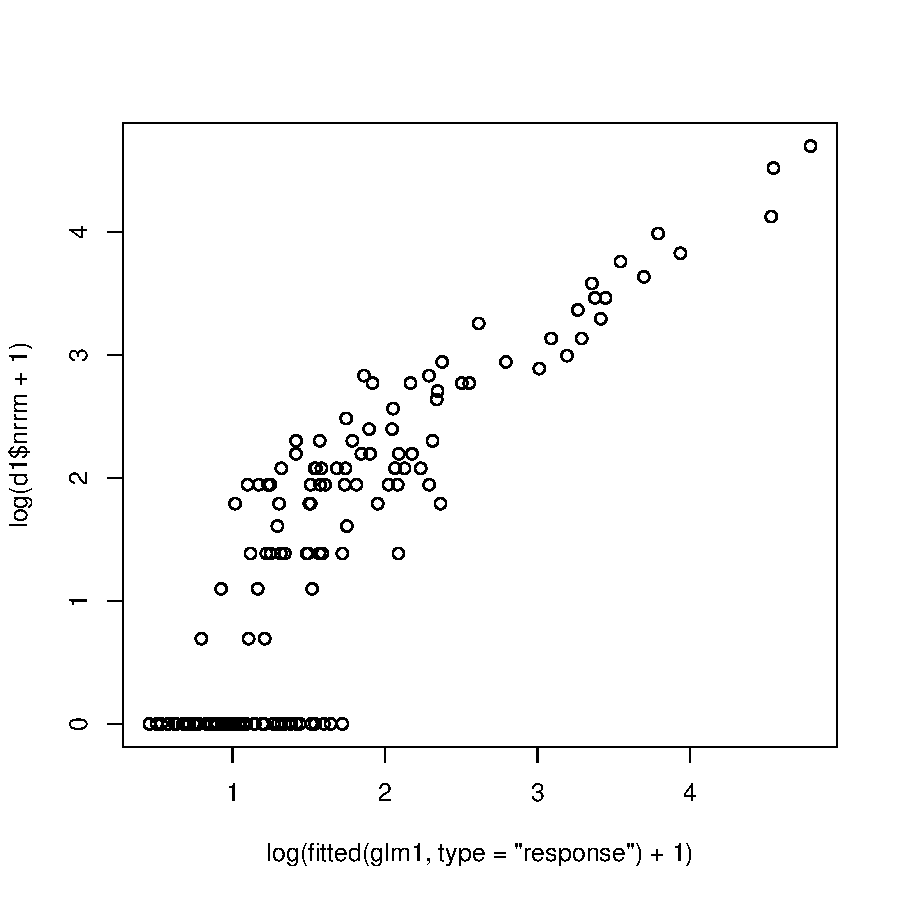
\includegraphics{HW08ZIPlogistic-glm1}

The plot of frequencies of number of individuals found in each location suggests that there are too many zeros. If we fit a glm with main effects and two-way interaction between continuous predictors, the plot of observed against fitted values also suggests that there are too many zeros.

Although we are not using the final model form for the counts, we are using a model that should produce relatively good predictions, because it is the full model.

\subsection{Modeling}

The residuals plot also suggests that there is a range of low fitted values for which the number of individuals found has too many zeroes. We decide to check this by fitting a zero-inflated Poisson model (ZIP) and testing if it is better than the glm.

Notice that the excessive frequency of zeros also results in a significant overdispersion. To test for overdispersion we fit a model using the quasipoisson family, which has one additional parameter to allow for a variance that is greater (by a constant factor) than the mean. Technically, the model development should be repeated with the new approach, but here we just test for overdispersion. The package AER has a function \verb!dispersiontest()! that performs a test of significance of overdispersion.
Using a quasipoisson family, however, does not fix the problem.

\begin{Schunk}
\begin{Sinput}
> glm2 <- glm(nrrm ~ river + road + cover + river:road + river:cover +
+               road:cover, family=quasipoisson, data=d1)
> plot(d1$nrrm~fitted(glm2, type="response"))
> summary(glm2)
\end{Sinput}
\begin{Soutput}
Call:
glm(formula = nrrm ~ river + road + cover + river:road + river:cover + 
    road:cover, family = quasipoisson, data = d1)

Deviance Residuals: 
    Min       1Q   Median       3Q      Max  
-3.4400  -1.7052  -0.6972   0.8537   3.6625  

Coefficients:
             Estimate Std. Error t value Pr(>|t|)    
(Intercept) -0.687277   0.482041  -1.426  0.15612    
river       -0.032729   0.045864  -0.714  0.47663    
road         0.103789   0.030837   3.366  0.00098 ***
cover        1.251678   0.706244   1.772  0.07847 .  
river:road   0.015314   0.003315   4.620 8.49e-06 ***
river:cover  0.014233   0.054571   0.261  0.79461    
road:cover   0.054315   0.048657   1.116  0.26618    
---
Signif. codes:  0 ‘***’ 0.001 ‘**’ 0.01 ‘*’ 0.05 ‘.’ 0.1 ‘ ’ 1

(Dispersion parameter for quasipoisson family taken to be 2.270525)

    Null deviance: 2546.64  on 149  degrees of freedom
Residual deviance:  395.63  on 143  degrees of freedom
AIC: NA

Number of Fisher Scoring iterations: 5
\end{Soutput}
\begin{Sinput}
> anova(glm2, test="Chisq")
\end{Sinput}
\begin{Soutput}
Analysis of Deviance Table

Model: quasipoisson, link: log

Response: nrrm

Terms added sequentially (first to last)


            Df Deviance Resid. Df Resid. Dev  Pr(>Chi)    
NULL                          149    2546.64              
river        1   351.94       148    2194.70 < 2.2e-16 ***
road         1  1390.02       147     804.68 < 2.2e-16 ***
cover        1   347.14       146     457.53 < 2.2e-16 ***
river:road   1    58.77       145     398.76 3.622e-07 ***
river:cover  1     0.28       144     398.48    0.7244    
road:cover   1     2.85       143     395.63    0.2629    
---
Signif. codes:  0 ‘***’ 0.001 ‘**’ 0.01 ‘*’ 0.05 ‘.’ 0.1 ‘ ’ 1
\end{Soutput}
\begin{Sinput}
> 1-pchisq(deviance(glm2),143) # excessive deviance; model needs to be improved
\end{Sinput}
\begin{Soutput}
[1] 0
\end{Soutput}
\begin{Sinput}
> par(mfrow=c(2,2))
> plot(glm2)
\end{Sinput}
\end{Schunk}
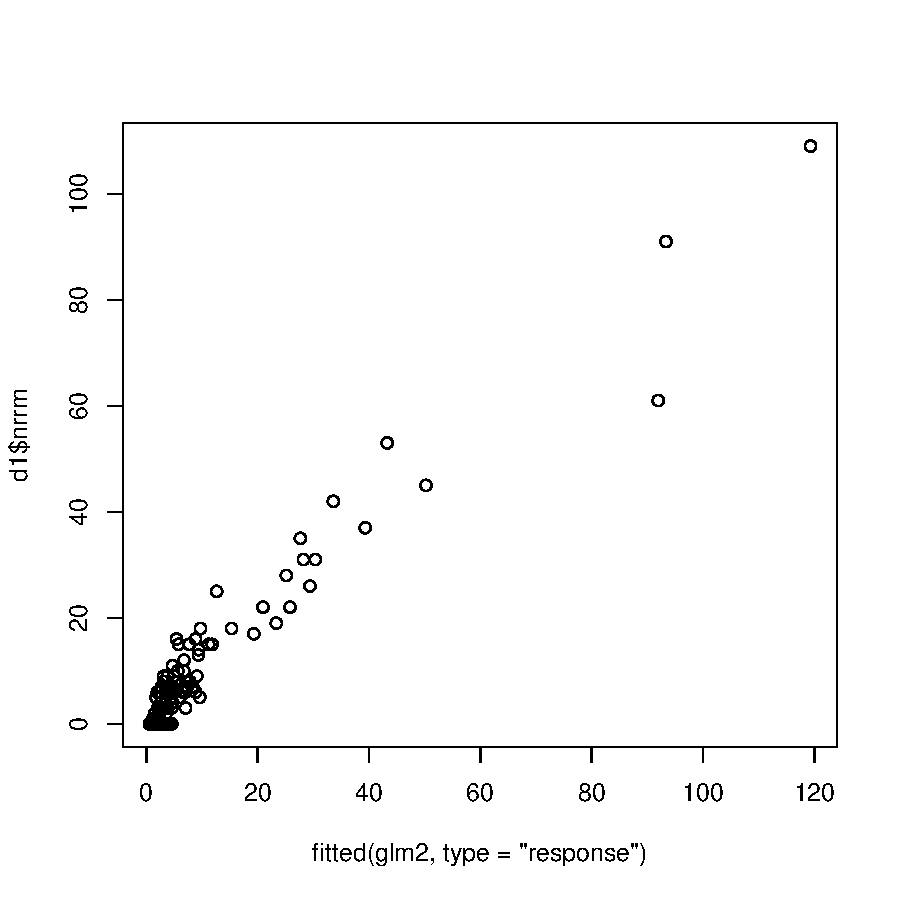
\includegraphics{HW08ZIPlogistic-glm2}

\subsection{ZIP}

In order to fit a ZIP we need to use the \verb!pscl! package. We start the modeling of the zeros by including all predictors in the zero inflation part of the model. Notice that the formula for \verb!zeroinfl()! has a vertical bar that separates the model for the counts (Poisson) from the model for the zero inflation (Binomial).
\begin{Schunk}
\begin{Sinput}
> library(pscl)
> zip1 <- zeroinfl(nrrm ~ river + road + cover + river:road + river:cover +
+                    road:cover | river + road + cover, data=d1)
> summary(zip1)
\end{Sinput}
\begin{Soutput}
Call:
zeroinfl(formula = nrrm ~ river + road + cover + river:road + river:cover + 
    road:cover | river + road + cover, data = d1)

Pearson residuals:
    Min      1Q  Median      3Q     Max 
-2.1497 -0.5164 -0.0130  0.1960  2.2691 

Count model coefficients (poisson with log link):
             Estimate Std. Error z value Pr(>|z|)    
(Intercept)  0.181298   0.374330   0.484  0.62815    
river       -0.082744   0.035701  -2.318  0.02047 *  
road         0.065150   0.024446   2.665  0.00770 ** 
cover        1.655472   0.535259   3.093  0.00198 ** 
river:road   0.018065   0.002681   6.738 1.61e-11 ***
river:cover  0.033397   0.035732   0.935  0.34997    
road:cover  -0.021370   0.038732  -0.552  0.58113    

Zero-inflation model coefficients (binomial with logit link):
            Estimate Std. Error z value Pr(>|z|)  
(Intercept) 23.06043   10.12254   2.278   0.0227 *
river       -0.05453    0.14603  -0.373   0.7088  
road        -4.22083    1.90981  -2.210   0.0271 *
cover       -3.06806    2.32337  -1.321   0.1867  
---
Signif. codes:  0 '***' 0.001 '**' 0.01 '*' 0.05 '.' 0.1 ' ' 1 

Number of iterations in BFGS optimization: 24 
Log-likelihood: -239.2 on 11 Df
\end{Soutput}
\end{Schunk}

The \verb!anova()! of glm1 indicated that \verb!river:cover! could be dropped from the count part. This is corroborated by the summary of zip1, where \verb!river:cover! has the highest probability among the interactions. The zero inflation part can be simplified by removing river.

\begin{Schunk}
\begin{Sinput}
> zip2 <- zeroinfl(nrrm ~ river + road + cover + river:road +
+                    road:cover | road + cover, data=d1)
> summary(zip2)
\end{Sinput}
\begin{Soutput}
Call:
zeroinfl(formula = nrrm ~ river + road + cover + river:road + road:cover | 
    road + cover, data = d1)

Pearson residuals:
    Min      1Q  Median      3Q     Max 
-2.1488 -0.5221 -0.0112  0.2394  2.2615 

Count model coefficients (poisson with log link):
             Estimate Std. Error z value Pr(>|z|)    
(Intercept) -0.025171   0.317156  -0.079  0.93674    
river       -0.061745   0.028298  -2.182  0.02911 *  
road         0.067010   0.024638   2.720  0.00653 ** 
cover        1.954520   0.437924   4.463 8.08e-06 ***
river:road   0.018062   0.002667   6.772 1.27e-11 ***
road:cover  -0.020157   0.038690  -0.521  0.60238    

Zero-inflation model coefficients (binomial with logit link):
            Estimate Std. Error z value Pr(>|z|)  
(Intercept)   24.088     12.251   1.966   0.0493 *
road          -4.522      2.329  -1.942   0.0522 .
cover         -3.188      2.560  -1.246   0.2129  
---
Signif. codes:  0 '***' 0.001 '**' 0.01 '*' 0.05 '.' 0.1 ' ' 1 

Number of iterations in BFGS optimization: 20 
Log-likelihood: -239.7 on 9 Df
\end{Soutput}
\end{Schunk}

We further simplify the model by eliminating road:cover from the count and cover from the zero inflation part.

\begin{Schunk}
\begin{Sinput}
> zip3 <- zeroinfl(nrrm ~ river + road + cover + river:road |
+                    road, data=d1)
> summary(zip3)
\end{Sinput}
\begin{Soutput}
Call:
zeroinfl(formula = nrrm ~ river + road + cover + river:road | road, data = d1)

Pearson residuals:
     Min       1Q   Median       3Q      Max 
-2.09269 -0.46801 -0.02856  0.24762  2.27802 

Count model coefficients (poisson with log link):
             Estimate Std. Error z value Pr(>|z|)    
(Intercept)  0.072247   0.266103   0.272  0.78601    
river       -0.060458   0.027769  -2.177  0.02947 *  
road         0.059896   0.021308   2.811  0.00494 ** 
cover        1.741514   0.130537  13.341  < 2e-16 ***
river:road   0.017758   0.002553   6.955 3.54e-12 ***

Zero-inflation model coefficients (binomial with logit link):
            Estimate Std. Error z value Pr(>|z|)   
(Intercept)   17.942      5.885   3.049  0.00230 **
road          -3.574      1.183  -3.020  0.00252 **
---
Signif. codes:  0 '***' 0.001 '**' 0.01 '*' 0.05 '.' 0.1 ' ' 1 

Number of iterations in BFGS optimization: 16 
Log-likelihood:  -241 on 7 Df
\end{Soutput}
\end{Schunk}

This model cannot be simplified any more, because all predictors are either significant or involved in a significant interaction. We can do a final test to make sure the model is not significantly worse than the initial full model.

\begin{Schunk}
\begin{Sinput}
> vuong(glm1,zip3) # the reduce model with the zero part is significantly better
\end{Sinput}
\begin{Soutput}
Vuong Non-Nested Hypothesis Test-Statistic: -8.076983 
(test-statistic is asymptotically distributed N(0,1) under the
 null that the models are indistinguishible)
in this case:
model2 > model1, with p-value 3.3194e-16 
\end{Soutput}
\begin{Sinput}
> # than the initial full model without zero inflation.
> plot(residuals(zip3, type="pearson") ~ fitted(zip3)) # no pattern -> OK
\end{Sinput}
\end{Schunk}
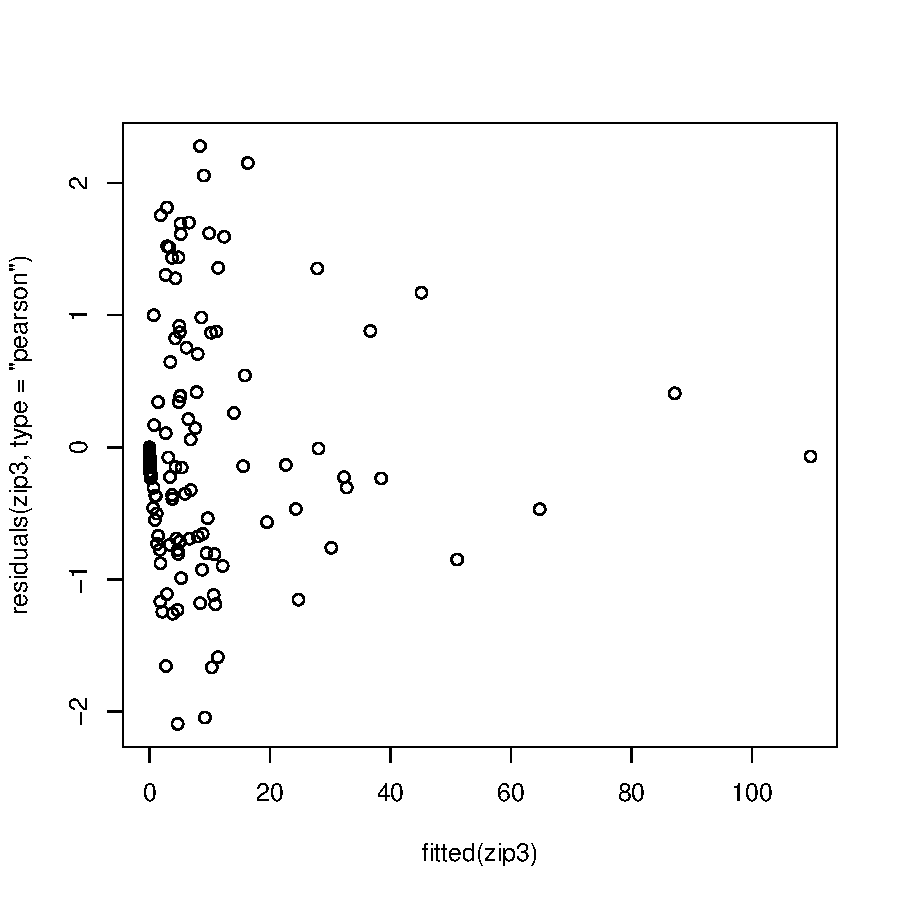
\includegraphics{HW08ZIPlogistic-val}

Now we have a final model that is reasonable we can interpret the results. Because the parameter estimates of the zero inflation and the count parts are each indirectly related to the actual observations through a link function, it is easiest to use a figure for the interpretation of results.

\subsection{Interpretation using graphs}

\begin{Schunk}
\begin{Sinput}
> # Predictions for various levels of cover and distance to river at average level of road
> mean(d1$road)
\end{Sinput}
\begin{Soutput}
[1] 6.444667
\end{Soutput}
\begin{Sinput}
> range(d1$river)
\end{Sinput}
\begin{Soutput}
[1]  0.5 14.7
\end{Soutput}
\begin{Sinput}
> range(d1$cover)
\end{Sinput}
\begin{Soutput}
[1] 0.008065092 0.921794636
\end{Soutput}
\begin{Sinput}
> p.data <- expand.grid(cover=seq(0.04,0.94,by=0.05), river=c(0,5,10,15),road=c(2,10,20))
> p.data$nrrm <- predict(zip3,newdata=p.data, type="response")
> ggplot(p.data, aes(x = cover, y = nrrm, colour = factor(river))) +
+   geom_point() +
+   geom_line() +
+   facet_wrap(~road) +
+   labs(x = "Cover", y = "Predicted number of rare mammal")
\end{Sinput}
\end{Schunk}
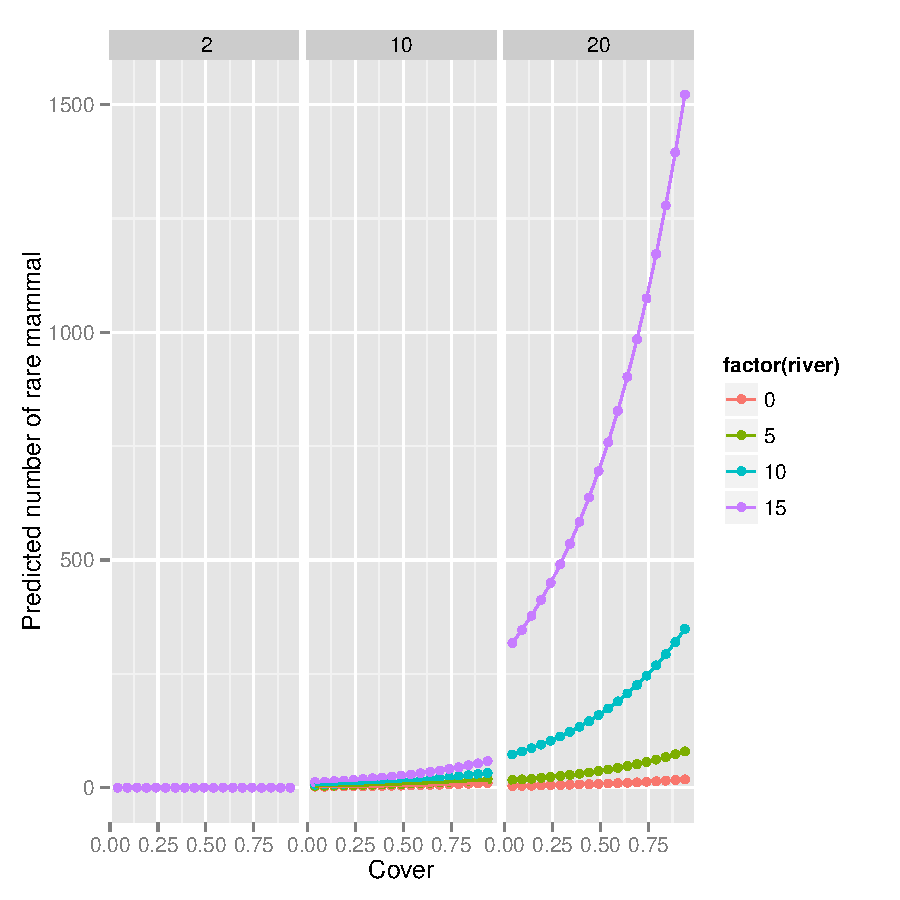
\includegraphics{HW08ZIPlogistic-011}

To explore the effect of road on zero inflation we can plot the predicted probability of "not found" or "not colonized" against road.


\begin{Schunk}
\begin{Sinput}
> plot(predict(zip3, type="zero") ~ d1$road)
\end{Sinput}
\end{Schunk}
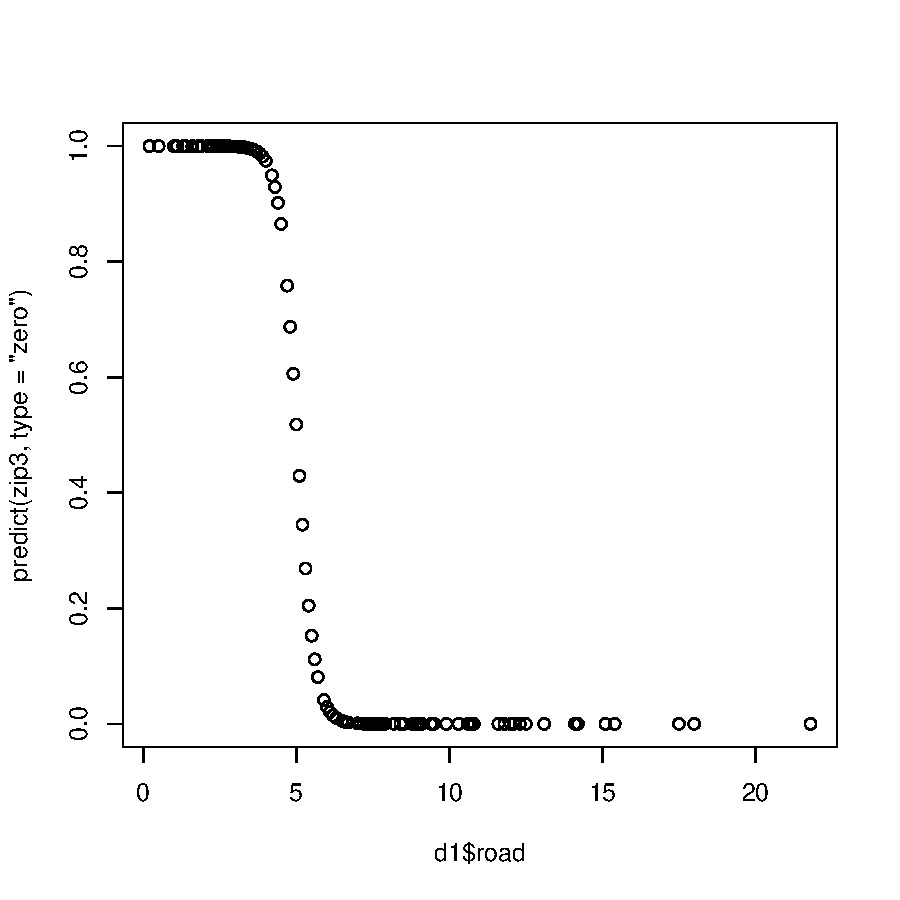
\includegraphics{HW08ZIPlogistic-012}

We see that the probability of a zero ("not colonized") declines as the distance to road increases.

\section {Zero Inflated Poisson: HW key}

This exercise is based on the same scenario as HW07 but the data have been change to include zero inflation. The main purpose of the exercise is to model data with zero inflation. All the code is provided. You are asked to run and document each chunk of code as grouped below.

For each chunk, write a comment describing the main purposes of the chunk. One to two sentences should be sufficient.
Interpret the result of each chunk as appropriate. For example, when the code produces a residual plot you would write whether there is any violation of assumptions suggested by the plot or not. For the final plots, how is abundance of the rare mammal affected by river, road and cover?
How does road affect the probability that the mammal found a particular location that might have suitable habitat? For this you need to interpret the zero inflation part of the model.

\subsection{Chunk 1}
\begin{Schunk}
\begin{Sinput}
> # Chunk 1
> d1 <- read.csv("../Examples/zeroinfl.txt", header=TRUE)
> library(car)
> library(ggplot2)
\end{Sinput}
\end{Schunk}
Data are read into R. Packages necessary for tests and graphics are loaded

\subsection{Chunk 2}
\begin{Schunk}
\begin{Sinput}
> # Chunk 2
> par(mfrow=c(1,1))
> plot(table(d1$nrrm))
\end{Sinput}
\end{Schunk}

Graphics window set to have one column and one row. A frequency plot of observations is made to inspect for excessive frequency of zeros. Indeed, the plot shows an overall excess of zeros relative to a Poisson distribution.

\subsection{Chunk 3}
\begin{Schunk}
\begin{Sinput}
> # Chunk 3
> glm1 <- glm(nrrm ~ river + road + cover + river:road + river:cover + road:cover, family=poisson, data=d1)
> plot(d1$nrrm~fitted(glm1, type="response"))
> summary(glm1)
\end{Sinput}
\begin{Soutput}
Call:
glm(formula = nrrm ~ river + road + cover + river:road + river:cover + 
    road:cover, family = poisson, data = d1)

Deviance Residuals: 
    Min       1Q   Median       3Q      Max  
-3.4400  -1.7052  -0.6972   0.8537   3.6625  

Coefficients:
            Estimate Std. Error z value Pr(>|z|)    
(Intercept) -0.68728    0.31990  -2.148  0.03168 *  
river       -0.03273    0.03044  -1.075  0.28225    
road         0.10379    0.02047   5.072 3.94e-07 ***
cover        1.25168    0.46870   2.671  0.00757 ** 
river:road   0.01531    0.00220   6.961 3.37e-12 ***
river:cover  0.01423    0.03622   0.393  0.69432    
road:cover   0.05432    0.03229   1.682  0.09256 .  
---
Signif. codes:  0 ‘***’ 0.001 ‘**’ 0.01 ‘*’ 0.05 ‘.’ 0.1 ‘ ’ 1

(Dispersion parameter for poisson family taken to be 1)

    Null deviance: 2546.64  on 149  degrees of freedom
Residual deviance:  395.63  on 143  degrees of freedom
AIC: 755.57

Number of Fisher Scoring iterations: 5
\end{Soutput}
\begin{Sinput}
> anova(glm1, test="Chisq")
\end{Sinput}
\begin{Soutput}
Analysis of Deviance Table

Model: poisson, link: log

Response: nrrm

Terms added sequentially (first to last)


            Df Deviance Resid. Df Resid. Dev  Pr(>Chi)    
NULL                          149    2546.64              
river        1   351.94       148    2194.70 < 2.2e-16 ***
road         1  1390.02       147     804.68 < 2.2e-16 ***
cover        1   347.14       146     457.53 < 2.2e-16 ***
river:road   1    58.77       145     398.76 1.768e-14 ***
river:cover  1     0.28       144     398.48   0.59527    
road:cover   1     2.85       143     395.63   0.09164 .  
---
Signif. codes:  0 ‘***’ 0.001 ‘**’ 0.01 ‘*’ 0.05 ‘.’ 0.1 ‘ ’ 1
\end{Soutput}
\begin{Sinput}
> 1-pchisq(deviance(glm1),143) # excessive deviance; model needs to be improved
\end{Sinput}
\begin{Soutput}
[1] 0
\end{Soutput}
\begin{Sinput}
> par(mfrow=c(2,2))
> plot(glm1)
\end{Sinput}
\end{Schunk}

A glm is used to start exploring the data with a plot of observed vs. predicted values. The fact that there is a range of predicted values for which zeros and greater values have a gap is also evidence of zero-inflation.
The \verb !anova()! shows that some terms may be dropped from the full model. The type I tests show that river is not significant, but its interaction with road is, so it is not a candidate for deletion. If we were performing variable selection, river:cover would be a reasonable first choice to be dropped. Under the assumption of Poisson distribution and the model, the deviance should have a $\chi^2$ distribution with n minus no. estimated parameters degrees of freedom. The observed value of the deviance is too extreme with respect to the $\chi^2$, which indicates that something in the model in not right. It could be overdispersion, zero inflation or an otherwise poor model. Residual plots are inspected for clues.

In order to see all residual plots in one window we specify 2 rows and two columns for the graphical output.

Residual plots show a string of observations whose residuals increase as the predicted values increase. Those are the excessively frequent zeros under the assumption of a single Poisson process whose mean increases smoothly with changing predictor values. The zeros tend to produce a "hump" or deviation from the flat line in the response residuals. There are a couple of observations that are overly influential and have high leverage. Those would be inspected for errors of transcription, typos and odd field conditions. This issue is not pursued in this exercise.

\subsection{Chunk 4}
\begin{Schunk}
\begin{Sinput}
> # Chunk 4
> library(AER)
> dispersiontest(glm1, trafo=1)
\end{Sinput}
\begin{Soutput}
	Overdispersion test

data:  glm1
z = 6.5148, p-value = 3.641e-11
alternative hypothesis: true alpha is greater than 0
sample estimates:
   alpha 
1.364721 
\end{Soutput}
\end{Schunk}

We use the \verb!dispersiontest()! function of the AER package to test for overdispersion. The test indicates that significant overdispersion is present. The \verb!trafo=1! argument can be dropped. The default results in a more direct test of the overdispersion coefficient =1.

\subsection{Chunk 5}
\begin{Schunk}
\begin{Sinput}
> # Chunk 5
> glm2 <- glm(nrrm ~ river + road + cover + river:road + 
+               river:cover + road:cover, family=quasipoisson, data=d1)
> plot(d1$nrrm~fitted(glm2, type="response"))
> summary(glm2)
\end{Sinput}
\begin{Soutput}
Call:
glm(formula = nrrm ~ river + road + cover + river:road + river:cover + 
    road:cover, family = quasipoisson, data = d1)

Deviance Residuals: 
    Min       1Q   Median       3Q      Max  
-3.4400  -1.7052  -0.6972   0.8537   3.6625  

Coefficients:
             Estimate Std. Error t value Pr(>|t|)    
(Intercept) -0.687277   0.482041  -1.426  0.15612    
river       -0.032729   0.045864  -0.714  0.47663    
road         0.103789   0.030837   3.366  0.00098 ***
cover        1.251678   0.706244   1.772  0.07847 .  
river:road   0.015314   0.003315   4.620 8.49e-06 ***
river:cover  0.014233   0.054571   0.261  0.79461    
road:cover   0.054315   0.048657   1.116  0.26618    
---
Signif. codes:  0 ‘***’ 0.001 ‘**’ 0.01 ‘*’ 0.05 ‘.’ 0.1 ‘ ’ 1

(Dispersion parameter for quasipoisson family taken to be 2.270525)

    Null deviance: 2546.64  on 149  degrees of freedom
Residual deviance:  395.63  on 143  degrees of freedom
AIC: NA

Number of Fisher Scoring iterations: 5
\end{Soutput}
\begin{Sinput}
> anova(glm2, test="Chisq")
\end{Sinput}
\begin{Soutput}
Analysis of Deviance Table

Model: quasipoisson, link: log

Response: nrrm

Terms added sequentially (first to last)


            Df Deviance Resid. Df Resid. Dev  Pr(>Chi)    
NULL                          149    2546.64              
river        1   351.94       148    2194.70 < 2.2e-16 ***
road         1  1390.02       147     804.68 < 2.2e-16 ***
cover        1   347.14       146     457.53 < 2.2e-16 ***
river:road   1    58.77       145     398.76 3.622e-07 ***
river:cover  1     0.28       144     398.48    0.7244    
road:cover   1     2.85       143     395.63    0.2629    
---
Signif. codes:  0 ‘***’ 0.001 ‘**’ 0.01 ‘*’ 0.05 ‘.’ 0.1 ‘ ’ 1
\end{Soutput}
\begin{Sinput}
> 1-pchisq(deviance(glm2),143) # excessive deviance; model needs to be improved
\end{Sinput}
\begin{Soutput}
[1] 0
\end{Soutput}
\begin{Sinput}
> par(mfrow=c(2,2))
> plot(glm2)
\end{Sinput}
\end{Schunk}

Pretending that we think the problem might be just overdispersion, we use a quasipoisson family and check if the problem is solved. The observed~predicted and residual plots still look like there are too many zeros for a range of predicted values, and the deviance is still too extreme for its df. So we decide to try a zero inflated model starting with the full model for the count and a model wit main effects for the zero inflation.

The \verb!summary(glm2)! shows that the type I significance of model terms is similar in relative terms to that of \verb!glm1! but lower in general. Because we will try a different type of model, it is not necessary to do variable selection.

\subsection{Chunk 6}
\begin{Schunk}
\begin{Sinput}
> # Chunk 6
> library(pscl)
> zip1 <- zeroinfl(nrrm ~ river + road + cover + river:road +
+                    river:cover + road:cover | river + road +
+                    cover, data=d1)
> summary(zip1)
\end{Sinput}
\begin{Soutput}
Call:
zeroinfl(formula = nrrm ~ river + road + cover + river:road + river:cover + 
    road:cover | river + road + cover, data = d1)

Pearson residuals:
    Min      1Q  Median      3Q     Max 
-2.1497 -0.5164 -0.0130  0.1960  2.2691 

Count model coefficients (poisson with log link):
             Estimate Std. Error z value Pr(>|z|)    
(Intercept)  0.181298   0.374330   0.484  0.62815    
river       -0.082744   0.035701  -2.318  0.02047 *  
road         0.065150   0.024446   2.665  0.00770 ** 
cover        1.655472   0.535259   3.093  0.00198 ** 
river:road   0.018065   0.002681   6.738 1.61e-11 ***
river:cover  0.033397   0.035732   0.935  0.34997    
road:cover  -0.021370   0.038732  -0.552  0.58113    

Zero-inflation model coefficients (binomial with logit link):
            Estimate Std. Error z value Pr(>|z|)  
(Intercept) 23.06043   10.12254   2.278   0.0227 *
river       -0.05453    0.14603  -0.373   0.7088  
road        -4.22083    1.90981  -2.210   0.0271 *
cover       -3.06806    2.32337  -1.321   0.1867  
---
Signif. codes:  0 '***' 0.001 '**' 0.01 '*' 0.05 '.' 0.1 ' ' 1 

Number of iterations in BFGS optimization: 24 
Log-likelihood: -239.2 on 11 Df
\end{Soutput}
\end{Schunk}

We loaded the \verb!pscl()! package for zero inflated models and try the first model. The model show a significant effect of road on zeros (longer distance fewer zeros). The interactions \verb!road:cover! and \verb!river:cover! are candidates for deletion in the count part but they have to be removed one at a time. For some reason, \verb!river:cover! was deleted first.

\subsection{Chunk 7}
\begin{Schunk}
\begin{Sinput}
> # Chunk 7
> zip2 <- zeroinfl(nrrm ~ river + road + cover + river:road + road:cover | road + cover, data=d1)
> summary(zip2)
\end{Sinput}
\begin{Soutput}
Call:
zeroinfl(formula = nrrm ~ river + road + cover + river:road + road:cover | 
    road + cover, data = d1)

Pearson residuals:
    Min      1Q  Median      3Q     Max 
-2.1488 -0.5221 -0.0112  0.2394  2.2615 

Count model coefficients (poisson with log link):
             Estimate Std. Error z value Pr(>|z|)    
(Intercept) -0.025171   0.317156  -0.079  0.93674    
river       -0.061745   0.028298  -2.182  0.02911 *  
road         0.067010   0.024638   2.720  0.00653 ** 
cover        1.954520   0.437924   4.463 8.08e-06 ***
river:road   0.018062   0.002667   6.772 1.27e-11 ***
road:cover  -0.020157   0.038690  -0.521  0.60238    

Zero-inflation model coefficients (binomial with logit link):
            Estimate Std. Error z value Pr(>|z|)  
(Intercept)   24.088     12.251   1.966   0.0493 *
road          -4.522      2.329  -1.942   0.0522 .
cover         -3.188      2.560  -1.246   0.2129  
---
Signif. codes:  0 '***' 0.001 '**' 0.01 '*' 0.05 '.' 0.1 ' ' 1 

Number of iterations in BFGS optimization: 20 
Log-likelihood: -239.7 on 9 Df
\end{Soutput}
\end{Schunk}

The new model show that we can drop \verb!road:cover! from the count part and \verb!cover! from the zero inflation part.

\subsection{Chunk 8}
\begin{Schunk}
\begin{Sinput}
> # Chunk 8
> zip3 <- zeroinfl(nrrm ~ river + road + cover + river:road |
+                    road, data=d1)
> summary(zip3)
\end{Sinput}
\begin{Soutput}
Call:
zeroinfl(formula = nrrm ~ river + road + cover + river:road | road, data = d1)

Pearson residuals:
     Min       1Q   Median       3Q      Max 
-2.09269 -0.46801 -0.02856  0.24762  2.27802 

Count model coefficients (poisson with log link):
             Estimate Std. Error z value Pr(>|z|)    
(Intercept)  0.072247   0.266103   0.272  0.78601    
river       -0.060458   0.027769  -2.177  0.02947 *  
road         0.059896   0.021308   2.811  0.00494 ** 
cover        1.741514   0.130537  13.341  < 2e-16 ***
river:road   0.017758   0.002553   6.955 3.54e-12 ***

Zero-inflation model coefficients (binomial with logit link):
            Estimate Std. Error z value Pr(>|z|)   
(Intercept)   17.942      5.885   3.049  0.00230 **
road          -3.574      1.183  -3.020  0.00252 **
---
Signif. codes:  0 '***' 0.001 '**' 0.01 '*' 0.05 '.' 0.1 ' ' 1 

Number of iterations in BFGS optimization: 16 
Log-likelihood:  -241 on 7 Df
\end{Soutput}
\end{Schunk}

The final model contains only terms that are significant. We want to make sure that the step-by-step term deletions did not lead to a model that is significantly worse than the full model. We use the \verb!vuong()! test do compare the full \verb!glm1! versus the final model.

\subsection{Chunk 9}
\begin{Schunk}
\begin{Sinput}
> # Chunk 9
> vuong(glm1,zip3) # the reduced model with the zero part is significantly
\end{Sinput}
\begin{Soutput}
Vuong Non-Nested Hypothesis Test-Statistic: -8.076983 
(test-statistic is asymptotically distributed N(0,1) under the
 null that the models are indistinguishible)
in this case:
model2 > model1, with p-value 3.3194e-16 
\end{Soutput}
\begin{Sinput}
>   #better than the initial full model without zero inflation.
> par(mfrow=c(1,1))
> plot(residuals(zip3, type="pearson") ~ fitted(zip3)) # no pattern -> OK
\end{Sinput}
\end{Schunk}

The plots of Pearson residuals vs. fitted values shows no patterns away from the horizontal 0. A plot of residuals vs. log(predicted) would provide a better view of the range of low predicted values.

\subsection{Chunk 10}
\begin{Schunk}
\begin{Sinput}
> # Chunk 10
> mean(d1$road)
\end{Sinput}
\begin{Soutput}
[1] 6.444667
\end{Soutput}
\begin{Sinput}
> range(d1$river)
\end{Sinput}
\begin{Soutput}
[1]  0.5 14.7
\end{Soutput}
\begin{Sinput}
> range(d1$cover)
\end{Sinput}
\begin{Soutput}
[1] 0.008065092 0.921794636
\end{Soutput}
\begin{Sinput}
> p.data <- expand.grid(cover=seq(0.04,0.94,by=0.05),
+                       river=c(0,5,10,15),road=c(2,10,20))
> p.data$nrrm <- predict(zip3,newdata=p.data, type="response")
> ggplot(p.data, aes(x = cover, y = nrrm, colour = factor(river))) +
+   geom_point() +
+   geom_line() +
+   facet_wrap(~road) +
+   labs(x = "Cover", y = "Predicted number of rare mammal")
\end{Sinput}
\end{Schunk}

The graphics show the effect of all predictors on counts observed, integrating the zero inflation and the count processes. Yet, it is pretty clear that at short distance to roads, most predictions are zero, regardless of the values of other predictors. 


\end{document}
